\input{notes.tex}

\usepackage{listings}

\iftoggle{dualscreen}{\setbeameroption{show notes on second screen=right}}{}
\begin{document}
\section{Lecture 3}
\subsection{Introduction}

\slide[Recall:]{
\vspace{-1em}
We saw how to use integration to solve the following first order ODEs\vfill
\[ y\p = f(t), \quad  y\p=f(y), \text{ and} \quad y'=g(y)f(t).\]\vfill
What happens if\enum{\item we cannot solve one of the integrals, or \item we get a more general ODE of the form $y'=f(y,t)$?}\vfill
\student{Exact analytical solutions are not always possible.\vfill \subitem{99.99\% of all the possible ODEs involve impossible integrals.}\vfill
Today we will build intuition around how to find approximate solutions.
}
}


\subsection{ Graphical intuition and the direction field}

\slide[Graphical intuition, whats does $y\p = f(y,t)$ mean?]{\vspace{-.5em}
\twomini[.58]{.4}{.59}{\vspace{-.5em}
\tikzplot{1}{3.25}{.5}{3.25}{t}{y(t)}{
\draw[thick, black] (0,3) .. controls (0,1) and (1,3) .. (3.5,-1);
\def\x0{1.6}
\def\y0{1.28}
\def\dx{.6}
\def\slope{-.77}
\def\spacer{.25}
\draw[ultra thick,->] (\x0-\dx,\y0-\dx*\slope) -- (\x0+\dx,\y0+\dx*\slope);
\node[vertex] at (\x0, \y0) {};
\draw[thick,|-|] (\x0-\dx,\y0+\dx*\slope-\spacer) -- (\x0+\dx,\y0+\dx*\slope-\spacer) node[midway, below]{$\Delta t$};
\draw[thick,|-|] (\x0-\dx-\spacer,\y0-\dx*\slope) -- (\x0-\dx-\spacer,\y0+\dx*\slope) node[midway, left]{$\Delta y$};
}


}
{

\[ \dd{y}{t} = f(y,t) \]

\student{
\vspace{.5em}
\algn{f(y,t) &= \text{slope of y(t) in the $(t,y)$-plane.}\\
&\approx\frac{\Delta y}{\Delta t}}



}
}
\uline{Slope Field Diagram:}\vfill
\student{ \enum{\item Draw an arrow with slope $f(y,t)$ for some points in the $(t,y)$-plane.\vfill
\item Stating from some initial condition(s), trace along with the arrows to get approximate solutions.} }
}

\presentonly{
\slide[Example: $y\p=2-y$, try different initial conditions]{
\twomini{.4}{.6}{

\resizebox{5.25cm}{7cm}{
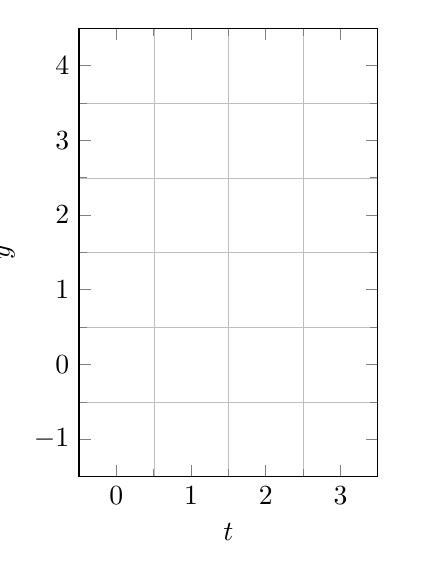
\begin{tikzpicture}\hspace{-.5cm}
\begin{axis}[
    xmin = -0.5, xmax = 3.5,
    ymin = -1.5, ymax = 4.5,
    zmin = 0, zmax = 1,
    grid=minor,
    grid style={line width=.1pt},
    major grid style={line width=.2pt},
    minor tick num=1,
    xtick = {0,1,2,3},
    ytick = {-1,0,1,2,3,4},
    axis equal image,
    view = {0}{90},
    xlabel={$t$},
    ylabel={$y$},
]



%    \addplot3[
%        quiver = {
%            u = {1/sqrt(1+(2-y)^2)},
%            v = {(2-y)/sqrt(1+(2-y)^2)},
%            scale arrows = 0.35,
%                every arrow/.append style={%
%                    line width=.1+\pgfplotspointmetatransformed/4000,
%                    -{Latex[length=0pt 5,width=0pt 3]}
%                }
%        },
%        -stealth,
%        domain = 0:3,
%        domain y = -1:4,
%        samples=16
%    ] {0};
%
\end{axis}

\end{tikzpicture}
}
}{
\enum{\item What type of solutions are possible? \student{\subitem{Monotonically increasing/decreasing}}\vspace{2em}
 \item What is $y(t)$ as $t\rightarrow\infty$?  \student{\subitem{Unique possibility: $y(t)\rightarrow2$ \item  $y=2$ is a stable steady state. }}\vspace{2em}
 \item What is the influence of the initial condition? \student{\subitem{If $y(0)>2$ decreasing solution. \item If $y(0)<2$ increasing solution.  \item If $y(0)=2$ constant solution. }}}
}

}
}

\fullonly{

\slide[Example: $y\p=2-y$, try different initial conditions]{
\twomini{.4}{.6}{

\resizebox{5.25cm}{7cm}{
\begin{tikzpicture}\hspace{-.5cm}
\begin{axis}[
    xmin = -0.5, xmax = 3.5,
    ymin = -1.5, ymax = 4.5,
    zmin = 0, zmax = 1,
    grid style={line width=.1pt},
    major grid style={line width=.2pt},
    xtick = {0,1,2,3},
    ytick = {-1,0,1,2,3,4},
    axis equal image,
    view = {0}{90},
    xlabel={$t$},
    ylabel={$y$},
]



    \addplot3[
        quiver = {
            u = {1/sqrt(1+(2-y)^2)},
            v = {(2-y)/sqrt(1+(2-y)^2)},
            scale arrows = 0.45,
                every arrow/.append style={%
                    line width=.1+\pgfplotspointmetatransformed/1500,
                    -{Latex[length=0pt 5,width=0pt 3]}
                }
        },
        -stealth,
        domain = 0:3,
        domain y = -1.1:4.1,
        samples=6
    ] {0};

\end{axis}

\end{tikzpicture}
}
}{
\enum{\item What type of solutions are possible? \student{\subitem{Monotonically increasing/decreasing}}\vspace{2em}
 \item What is $y(t)$ as $t\rightarrow\infty$?  \student{\subitem{Unique possibility: $y(t)\rightarrow2$ \item  $y=2$ is a stable steady state. }}\vspace{2em}
 \item What is the influence of the initial condition? \student{\subitem{If $y(0)>2$ decreasing solution. \item If $y(0)<2$ increasing solution.  \item If $y(0)=2$ constant solution. }}}
}

}

}

\begin{frame}[fragile]
\frametitle{slopefield.m}

A convenient MATLAB function that will plot slopefields for you!\vfill 
\textcolor{black}{\small
\lstinputlisting[language=Matlab, frame=single]{matlab_scripts/slopefield.m}
}
\vfill
Copy-paste into a file called \alert{slopefield.m} in your MATLAB development environment
\end{frame}

\begin{frame}[fragile]
\vfill
\frametitle{\ex{$y'=e^{2y}$}}

\twomini[.7]{.4}{.55}{
\textcolor{black}{
\lstinputlisting[language=Matlab, frame=single]{matlab_scripts/slopefield_ex1.m}
}
}{
\includegraphics[width=.95\columnwidth]{images/blowup_field.pdf}
}\vfill
Note: The slope is positive for all values of y. Blowup happens for all initial conditions.
\end{frame}



\begin{frame}[fragile]
\vfill
\frametitle{\ex{$y'=\frac{x^2}{y}$}}

\twomini[.7]{.4}{.55}{
\textcolor{black}{
\lstinputlisting[language=Matlab, frame=single]{matlab_scripts/slopefield_ex2.m}
}
}{
\includegraphics[width=.95\columnwidth]{images/slopefield_ex2.pdf}
}\vfill
Trace a solution backwards from $y(0)=1$.\vfill
Why does the solution not exist for $x<-\sqrt[3]{\nicefrac32}$? \vfill 

\centering \student{$f(x,y)$ is discontinous $y=0$}
\vfill
\end{frame}

\subsection{Existence and uniqueness}

\slide[Picard's Theorem]{
A \uline{unique} solution to
\vfill
 \[y'=f(t,y),\quad \text{with } y(t_0)=y_0\] 
\vfill
exists for t near $t_0$ if\vfill \enum{ \item $f(t,y)$ is continuous (as a function of two variables) and \item $\nicefrac{\partial f}{\partial y}$ exists and is continuous near $(t_0,y_0)$.}

\vfill

}

\slide[\ex{$y'=2\sqrt{|y|}$, with y(0)=0}]{
\twomini[.6]{.6}{.4}{
Analytically, we find 2 solutions
\enum{\item By inspection: \[y(t)=0\] \item Integrate for positive and negative $y$ separately: \[y(t)=\begin{cases}  t^2 & t\geq0 \\ -t^2 & t<0 \end{cases}\] }
}{\includegraphics[width=.95\columnwidth]{images/1-3-sqrt-sol-mbx.pdf}}
\vfill
\student{Picard's uniqueness theorem does not apply, because $\pd{}{y}2\sqrt{|y|}$ does not exist at $y=0$.}
}

\end{document}